% Drawing 148/01-3 -- folder 148, batch 01, archive page 8 (PDF page 9).
% Transcription: à gauche, un croquis : l'hexagone de sommets $\pm 1$, $\pm\zeta$, $\pm\bar{\zeta}$, le réseau et ses points marqués
% Kind: hexagon of the Eisenstein lattice with marked points. Method 2 (schematic redraw from the facsimile). Status: ok.
% Notes: Re-read on a tight crop of p. 8. The hexagon with vertices zeta (upper left), -zeta-bar (upper right), 1 (right), -zeta (lower right), zeta-bar (lower left) and the unlabelled vertex -1 (left), its three diagonals through the centre (the half towards zeta heavy with an arrow, the half towards 1 heavy with an arrow); the lattice lines through the six ringed points of the next shell, drawn as a star of David (two triangles), the ringed points, the small lattice points and an open point below the centre; pencil lines from a point above the hexagon down to the centre, to zeta and towards -zeta-bar, and a pencil stroke at the upper left. Labels read on the crop as zeta with a bar or a minus sign (the bars are short strokes above the letters); -1 is not written. Stray pencil strokes to the right belong to another sketch and are left out.
% Coordinates: 1 unit = 1 mm = 1/100 of the crop width (bbox in page fractions: [0.14, 0.37, 0.35, 0.53]).
% Redrawn by Claude (claude-opus-5-5), issue #73, 2026-11-07; not checked by a human; not compiled (no TeX in the session).
% Rights: reproduces part of the work -- behind RENDER_TRANSCRIPTS, never published by itself.
\documentclass[tikz,border=3pt]{standalone}
\usepackage{amsmath,amssymb}
\usetikzlibrary{patterns,arrows.meta}
\tikzset{pencil/.style={black!45}, struck/.style={black!35}, mark/.style={circle,draw,inner sep=1.3pt}, pt/.style={circle,fill,inner sep=0.9pt}, opt/.style={circle,draw,fill=white,inner sep=1.1pt}}
\begin{document}
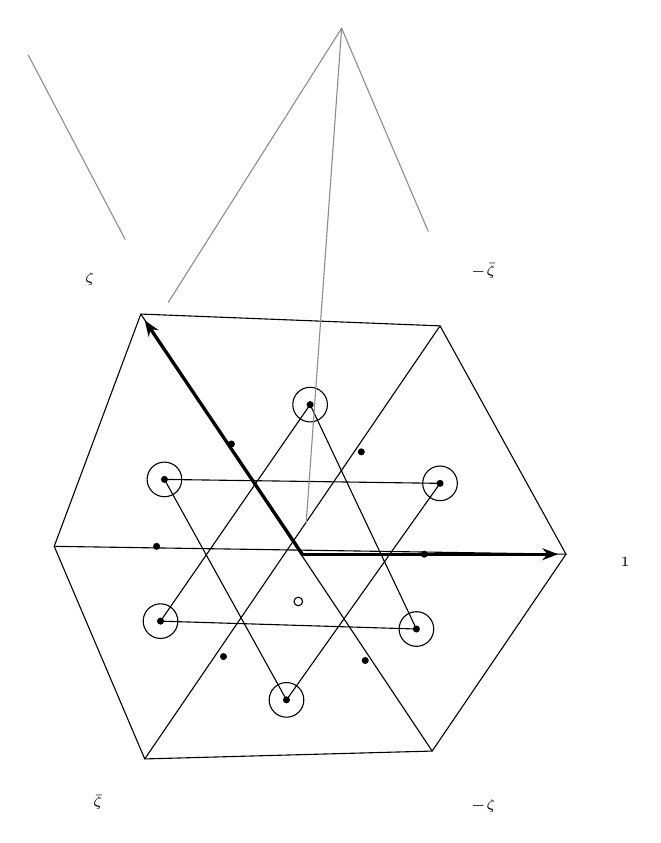
\begin{tikzpicture}[x=1mm,y=1mm,line cap=round,line join=round,font=\scriptsize]
\draw (30.5,-39) -- (68.5,-40.5) -- (84.5,-69.5) -- (67.5,-94.5) -- (31,-95.5) -- (19.5,-68.5) -- cycle;
\draw (30.5,-39) -- (67.5,-94.5);
\draw (68.5,-40.5) -- (31,-95.5);
\draw (19.5,-68.5) -- (84.5,-69.5);
\draw[very thick,-{Stealth[length=2mm]}] (51,-69.5) -- (31,-39.8);
\draw[very thick,-{Stealth[length=2mm]}] (51,-69.5) -- (83.5,-69.5);
\draw (33.5,-60) -- (68.5,-60.5) -- (49,-88) -- cycle;
\draw (52,-50.5) -- (65.5,-79) -- (33,-78) -- cycle;
\draw (52,-50.5) circle[radius=2.2];
\draw (33.5,-60) circle[radius=2.2];
\draw (68.5,-60.5) circle[radius=2.2];
\draw (33,-78) circle[radius=2.2];
\draw (65.5,-79) circle[radius=2.2];
\draw (49,-88) circle[radius=2.2];
\node[pt] at (52,-50.5) {};
\node[pt] at (33.5,-60) {};
\node[pt] at (68.5,-60.5) {};
\node[pt] at (33,-78) {};
\node[pt] at (65.5,-79) {};
\node[pt] at (49,-88) {};
\node[pt] at (32.5,-68.5) {};
\node[pt] at (66.5,-69.5) {};
\node[pt] at (58.5,-56.5) {};
\node[pt] at (41,-82.5) {};
\node[pt] at (59,-83) {};
\node[pt] at (42,-55.5) {};
\node[opt] at (50.5,-75.5) {};
\draw[pencil] (56,-2.7) -- (51.5,-65.5);
\draw[pencil] (56,-2.7) -- (34,-37.5);
\draw[pencil] (56,-2.7) -- (67,-28.5);
\draw[pencil] (16.2,-6.1) -- (28.5,-29.5);
\node[inner sep=1pt] at (24,-34.5) {\tiny $\zeta$};
\node[inner sep=1pt] at (74,-33.5) {\tiny $-\bar\zeta$};
\node[inner sep=1pt] at (25,-101) {\tiny $\bar\zeta$};
\node[inner sep=1pt] at (74,-101.5) {\tiny $-\zeta$};
\node[inner sep=1pt] at (92,-70.5) {\tiny $1$};
\end{tikzpicture}
\end{document}
